\documentclass{../industrial-development}
\graphicspath{{04-software-development-practices/}}

\title{Методологии разработки ПО}
\author{Филонов Дмитрий Русланович}
\date{}

\begin{document}

\begin{frame}
  \titlepage
\end{frame}

\begin{frame}{План лекции}
  \tableofcontents
\end{frame}

\section{Ретроспектива}
\subsection{}

\begin{frame} \frametitle{}
  \begin{block}{Важный факт}
    Большинство методологий есть результат организации \alert{основных} бизнес-процессов по разработке ПО или процессов \alert{управления} компанией, которая занимается разработкой ПО.
  \end{block}
Выделяются следующие \alert{основные} для разработки ПО бизнес-процессы:
\centerline{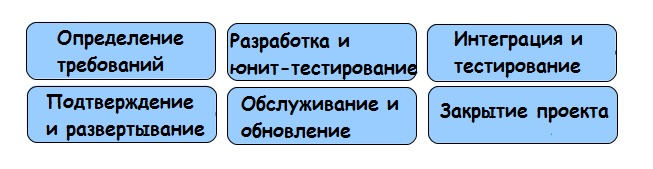
\includegraphics[width=1.10\textheight]{BP.png}} 
\end{frame}

\begin{frame} \frametitle{Waterfall}
  \begin{block}{}
    Классическая традиционная и методика разработки ПО, активно развивающейся с 1980.
  \end{block}
 \centerline{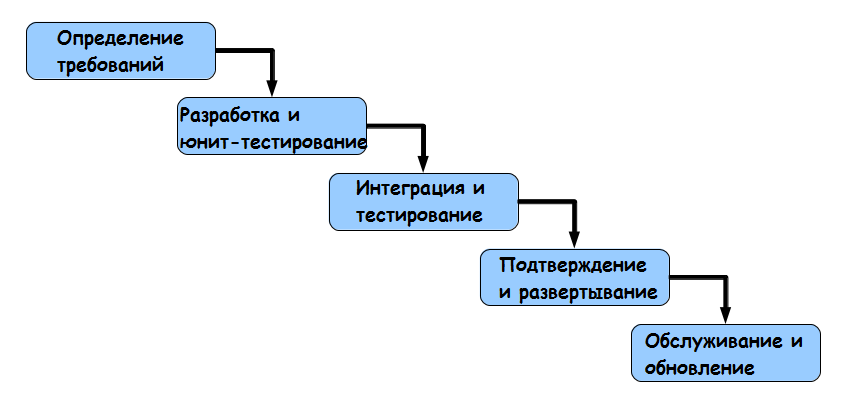
\includegraphics[height=0.6\textheight]{w1.png}}
\end{frame}

\lecturenotes
Говоря о гибкой методологии разработки ПО необходимо в начале упомянуть о некоторых предшествующих им методиках разработки. Одной из таких методик является модель Waterfall «метод водопада» относящийся к классическому пониманию разработки ПО и являющейся одной из главных примеров традиционных методик. Модель водопада зародилась и развивалась с 1980 г.
Весь процесс производства является жестким и линейным, имеет четкие цели для каждого этапа, новая фаза начинается по завершению предыдущей. Преимущества водопадной методологии---децентрализация и строгий контроль над сроками и качеством исполнения~\cite{Winston}.


\begin{frame} 
  \begin{block}{Преимущества Waterfall}
	\begin{itemize}
  \item Линейность 
	\item Последовательность
	\item Строгий контроль над исполнением и сроками различных стадий разработки
  \item Поэтому, процесс разработки в <<Waterfall>> является простым и наглядным для понимания
  \end{itemize}
	\end{block}
\end{frame}

\begin{frame} \frametitle{Удивительно, но}
\begin {block}{Недостатки Waterfall}
  \begin{itemize}
  \item Линейность 
  \item Последовательность 
	\item Строгий контроль над исполнением и сроками различных стадий разработки
  \end{itemize}
\end {block}
\end{frame}

\begin{frame} \frametitle{Недостатки Waterfall}
Линейность и последовательность игнорируют следующие важные факторы:
  \begin{itemize}
  \item Динамические изменения в требованиях заказчика
  \item Проблемы с откатыванием процесса разработки назад
	\item Временные простои сотрудников в рамках 1 проекта
	\item Каждый следующий этап разработки разворачивается только после получения строго определенной спецификации предыдущего
	 \end{itemize}
\begin {block}{}Все эти факторы ведут к \alert {росту издержек} или \alert{потерям времени}.\end {block}
\end{frame}


\begin{frame} \frametitle{Проблема Waterfall}
\begin {block}{}
Определенно стоит быть более \alert{гибким к внешним изменениям}. Ведь ко времени окончательной реализации заказчику потребуется уже совсем \alert{другой продукт}\dots
\end {block}
\end{frame}
\lecturenotes
На практике Waterfall часто не оправдывает ожиданий, поскольку игнорирует динамические изменения. Так, после тестирования очень сложно откатить процесс и заложить функции, не учтенные на стадии разработки. Waterfall неэффективен ещё и потому, что предполагает временные простои сотрудников в рамках одного проекта. ~\cite{MethodolyComparison}Тестирование проводится только в конце разработки, хотя проблемы, найденные на этом этапе — это дорогостоящие исправления. В последние 2 декады 20 столетия стоимость издержек росла экспоненциально на каждом этапе разработки. Однако, есть и модификации, данной методологии, которые устраняют эти недостатки. Об этих модификациях можно узнать в труде Профессора Винстона В. Ройса   <<MANAGING THE DEVELOPMENT OF LARGE SOFTWARE SYSTEMS>>. Одним из таких приемов является техника <<сделай это дважды>>, которая заключается в рекурсивном использовании Waterfall внутри каждого из этапов, что очень похоже на главную особенность Scrum - гибкой методологии, формально сформировавшейся лишь в 21 веке. Авторам даже удалось реализовать <<откаты назад>> в рамках данной модели~\cite[с.~335--338]{Winston}, однако на каждую дополнительную технику модернизации процесса тратятся дополнительные средства заказчика, тем не менее их рост более линейный, нежели экспоненциальный. ~\cite{Winston}.


\begin{frame} \frametitle{}
\begin {block}{Waterfall перестает действовать в следющей ситуации}
Если потребности заказчика:
 \begin{itemize}
\item Постоянно изменяются в \alert{динамическом бизнесе}
\item Не совсем или не до-конца ясны на \alert{начальном этапе}
\item Его финансы \alert {ограничены}
\end{itemize}
То становится не ясно---какой тактики и методики придерживаться?
\end {block}
\end{frame}

\begin{frame} \frametitle{RAD}
  \begin{itemize}
  \item Основной девиз---<<Сразу к делу, а там разберемся>>
  \item Эффективен только с простыми заказами, требования к которым описываются интерфейсом пользователя 
	\item Основной инструмент разработчика - graphical user interface builder (GUI builder)
	\item Не требует строго определенную спецификацию, установленной до входа в очередную фазу разработки
	\item RAD подчеркивают адаптивность и необходимость корректировки требований в ответ на новые знания, полученные по мере продвижения проекта.
	\item Прототипы часто используются в дополнение или иногда даже вместо спецификаций.
  \end{itemize}

\end{frame}

\begin{frame} \frametitle{}
\begin {block}{Недостатки RAD}
Отсутствие \alert {масштабируемости} RAD и неприменимость его в крупных проектах и гигантских компаниях послужило толчком к развитию новых, более гибких и в то же время структурированных подходов.
\end {block}
\end{frame}	
	
\lecturenotes
Основной девиз RAD---<<Сразу к делу, а там разберемся>>. Данная методология работает эффективно только с относительно простыми проектами, где требования заказчика по-большей части определяются интерфейсом.
Потому RAD не требует строго определенную спецификацию, которая должна быть установлена до входа в очередную фазу разработки.
Подходы RAD подчеркивают адаптивность и необходимость корректировки требований в ответ на новые знания, полученные по мере продвижения  проекта. Прототипы часто используются в дополнение или иногда даже вместо спецификаций.
Однако, отсутствие \alert {масштабируемости} RAD и неприменимость его в крупных проектах и гигантских компаниях послужило толчком к развитию новых, более гибких и в то же время структурированных подходов.
Основной инструмент разработчика---graphical user interface builder (GUI builder).
Другие подходы к быстрому развитию включают Agile-методы и спиральную модель.~\cite{MethodolyComparison}

	
\begin{frame} \frametitle{Cпиральная методология}
Основное внимание уделяется \alert{оценке рисков} и \alert{минимизации проектного риска} путем
\begin{itemize}
		\item разбиения проект на более мелкие сегменты
		\item обеспечения легкости для внесения изменений изменений 
\end{itemize}		
\begin{block}{}
Каждый цикл спирали включает в себя одну и ту же последовательность шагов как для концепции работы общего проекта до так и для его каждого сегмента.
\end{block} 
\end{frame}

\begin{frame} \frametitle{Cпиральная методология}
  \centerline{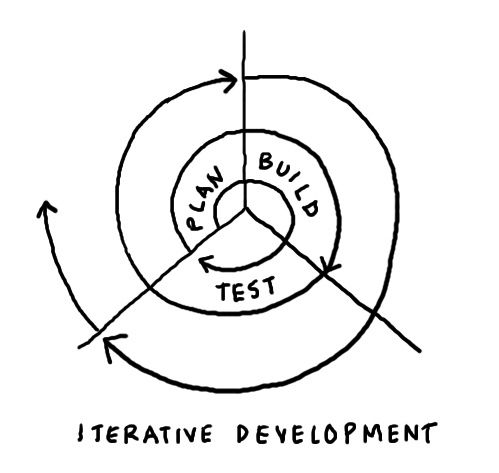
\includegraphics[height=0.9\textheight]{s1.png}}
\end{frame}

\begin{frame} \frametitle{Cпиральная методология}

  \begin{itemize}
 	\item Каждый оборот спирали пересекает четыре основных квадранта:
	\begin{itemize} 
	\item Определение цели, альтернативы и ограничения итерации 
	\item Оценивание альтернатив; Выявление и устранение рисков
	\item Разработка и проверка результатов итерации
	\item Планирование следующей итерацию
	\end{itemize}
	\item Каждый цикл начинается с переговоров с заинтересованной стороной их условиями и заканчивается обзором и демонстрацией выполненных требований. 
  \end{itemize}
\end{frame}

\begin{frame} \frametitle{Cпиральная методология}
  \centerline{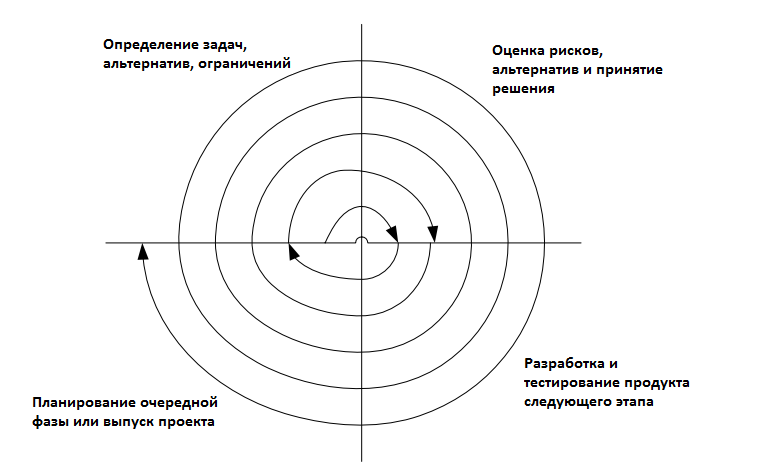
\includegraphics[height=0.9\textheight]{s2.png}}
\end{frame}


\begin{frame} \frametitle{Cпиральная методология}
  \centerline{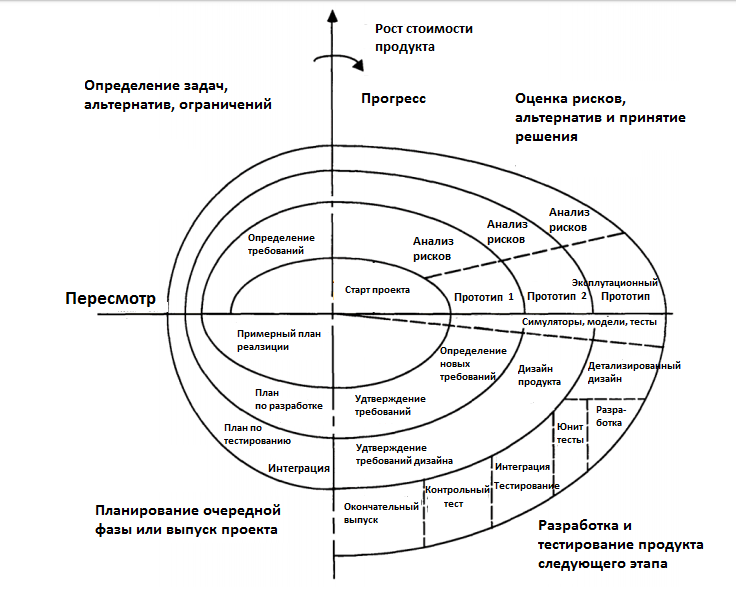
\includegraphics[height=0.80\textheight]{s3.png}}
\end{frame}

\lecturenotes
В 1988 году Барри Бём официально опубликовал новую методологию разработки ПО назвав её «Спиральная модель». Она сочетает в себе некоторые ключевые аспекты модели Waterfall и RAD. Также Бём включил в неё преднамеренный итеративный анализ рисков, особенно подходящий для крупномасштабных сложных систем.
Основное внимание уделяется оценке рисков и минимизации проектного риска, разбивая проект на более мелкие сегменты и обеспечивая легкость изменений в процессе разработки, а также предоставлию возможности оценивать риски и взвешивать рассмотрение продолжения проекта на протяжении всего жизненного цикла~\cite{MethodolyComparison}.
Каждый цикл включает в себя одну и ту же последовательность шагов как для концепции работы общего проекта до так и для его каждого сегмента. Каждая оборот спирали пересекает четыре основных квадранта: 
\begin{enumerate}
	\item Определение цели, альтернативы и ограничения итерации
	\item Оценивание альтернатив; Выявление и устранение рисков
	\item Разработка и проверка результатов итерации
	\item Планирование следующую итерацию
\end{enumerate}
Начинайте каждый цикл с переговоров с заинтересованной стороной (заказчиком) и их условиями и заканчивайте каждый цикл обзором и демонстрацией выполненных требований~\cite{Boehm}. 


\section{Возникновение и главные особенности Agile}

\begin{frame} \frametitle{Причины возникновения Agile}
Тенеденция сделать процесс разработки 
 \begin{itemize}
  \item более гибким
	\item снизить издержки
	\item сэкономить время
	\item привлечь новых клиентов 
	\end{itemize}
\begin{block}{}
способствовала тому, что в феврале 2001 в штате Юта США в романтичном месте под названием Snowbird был выпущен «Манифест гибкой методологии разработки программного обеспечения» (Agile). 
\end {block}
\end {frame}


\begin{frame} \frametitle{Возникновение Agile} 
Agile манифест был одобрен и подписан представителями методологий: 
\begin{itemize}
  \item eXtreme Programming (XP)
	\item Scrum
	\item Lean & etc.
	\end{itemize}
Гибкая методология разработки использовалась многими компаниями и до принятия манифеста, однако вхождение Agile-разработки в массы произошло именно после этого события.
\end{frame}


\begin{frame} \frametitle{12 принципов  Agile}
\begin{enumerate}
\item[1] Наивысшим приоритетом является удовлетворение потребностей 
заказчика, благодаря регулярной и ранней поставке ценного программного 
обеспечения.
\item[2] Изменение требований приветствуется, даже на поздних стадиях разработки. 
Agile-процессы позволяют использовать изменения для обеспечения заказчику
конкурентного преимущества.
\item[3] Работающий продукт следует выпускать как можно чаще, с периодичностью 
от пары недель до пары месяцев.
\item[4] На протяжении всего проекта разработчики и представители бизнеса должны 
ежедневно работать вместе.
\end{enumerate}
\end{frame}


\begin{frame} \frametitle{12 принципов  Agile}
\begin{enumerate}

\item[5] Над проектом должны работать мотивированные профессионалы. Чтобы 
работа была сделана, создайте условия, обеспечьте поддержку и полностью 
доверьтесь им.
\item[6] Непосредственное общение является наиболее практичным и эффективным 
способом обмена информацией как с самой командой, так и внутри команды.
\item[7] Работающий продукт — основной показатель прогресса.
\item[8] Инвесторы, разработчики и пользователи должны иметь возможность 
поддерживать постоянный ритм.
\end{enumerate}
\end{frame}

\lecturenotes

\begin{frame} \frametitle{12 принципов  Agile}
\begin{itemize}
\item[9] Постоянное внимание к техническому совершенству и качеству 
проектирования повышает гибкость проекта.
\item[10] Простота — искусство минимизации лишней работы — крайне необходима.
\item[11] Самые лучшие требования, архитектурные и технические решения рождаются 
у самоорганизующихся команд.
\item[12] Команда должна систематически анализировать возможные способы 
улучшения эффективности и соответственно корректировать  стиль своей работы.
\end{itemize}
\end{frame}

\begin{frame} \frametitle{Следствие 12 принципов}
\begin{itemize}
\item \alert{Люди и их взаимодействие}  важнее процессов и инструментов; 
\item \alert{Готовый продукт} важнее документации по нему; 
\item \alert{Сотрудничество с заказчиком} важнее жестких контрактных ограничений; 
\item \alert{Реакция на изменения} важнее следования плану.
\end{itemize}
\begin{block}{}
То есть, не отрицая важности того, что справа, сторонники гибкой методологии все-таки больше ценят то, что слева.
\end{block}
\end{frame}


\lecturenotes
Попытка разрешить вышеупомянутый вопрос послужил причиной тому, что в феврале 2001 в штате Юта США в романтичном месте под названием Snowbird был выпущен «Манифест гибкой методологии разработки программного обеспечения» (Agile). Он являлся альтернативой управляемым документацией традиционным «тяжеловесным» практикам разработки программного обеспечения, таким как «Waterfall», являвшимся уже золотым стандартом разработки в то время. Agile манифест был одобрен и подписан представителями методологий: экстремального программирования, Scrum, Lean. Гибкая методология разработки использовалась многими компаниями и до принятия манифеста, однако вхождение Agile-разработки в массы произошло именно после этого события.
Ниже представлены основные 12 принципов из манифеста гибкой методологии разработки ПО:
\end{block}
\begin{enumerate}
\item[1] Наивысшим приоритетом является удовлетворение потребностей 
заказчика, благодаря регулярной и ранней поставке ценного программного 
обеспечения.
\item[2] Изменение требований приветствуется, даже на поздних стадиях разработки. 
Agile-процессы позволяют использовать изменения для обеспечения заказчику
конкурентного преимущества.
\item[3] Работающий продукт следует выпускать как можно чаще, с периодичностью 
от пары недель до пары месяцев.
\item[4] На протяжении всего проекта разработчики и представители бизнеса должны 
ежедневно работать вместе.
\item[5] Над проектом должны работать мотивированные профессионалы. Чтобы 
работа была сделана, создайте условия, обеспечьте поддержку и полностью 
доверьтесь им.
\item[6] Непосредственное общение является наиболее практичным и эффективным 
способом обмена информацией как с самой командой, так и внутри команды.
\item[7] Работающий продукт — основной показатель прогресса.
\item[8] Инвесторы, разработчики и пользователи должны иметь возможность 
поддерживать постоянный ритм.
\item[9] Постоянное внимание к техническому совершенству и качеству 
проектирования повышает гибкость проекта.
\item[10] Простота — искусство минимизации лишней работы — крайне необходима.
\item[11] Самые лучшие требования, архитектурные и технические решения рождаются 
у самоорганизующихся команд.
\item[12] Команда должна систематически анализировать возможные способы 
улучшения эффективности и соответственно корректировать  стиль своей работы\cite{Scrum}.
\end{enumerate}
\end{itemize}
\begin{block}
Проанализировав данные принципы и осознав преимущества новых гибких  методик, авторы пришли к следующим важным выводам:
\end{block}
\begin{itemize}
\item \alert{Люди и их взаимодействие}  важнее процессов и инструментов; 
\item \alert{Готовый продукт} важнее документации по нему; 
\item \alert{Сотрудничество с заказчиком} важнее жестких контрактных ограничений; 
\item \alert{Реакция на изменения} важнее следования плану.
\end{itemize}
\begin{block}
То есть, не отрицая важности того, что справа, сторонники гибкой методологии все-таки больше ценят то, что слева~\cite{Agile}.
\end{block}


\section{Scrum}

\subsection{Определение}
\begin{frame} \frametitle{Определение}
  \begin{block}{Scrum}
Это один из подходов гибкой разработки ПО. Основан на эмпирическом методе и предназначен для разработки продуктов высокой ценности в запутанной среде.
  \centerline{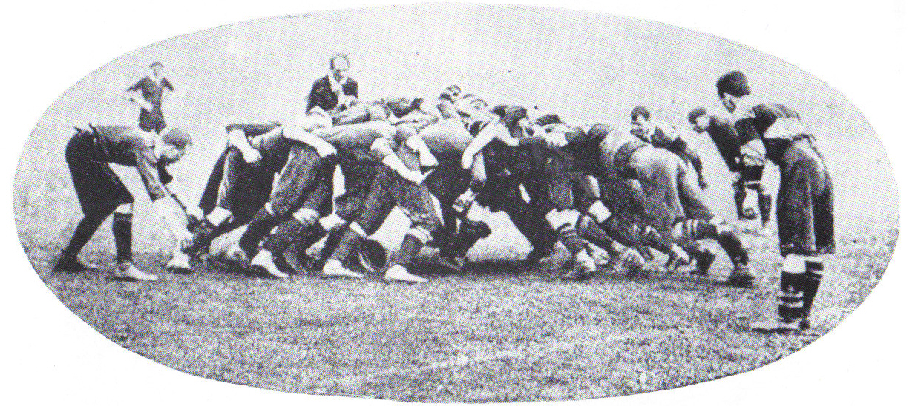
\includegraphics[height=0.85\textheight]{sc1.png}}
	\end{block}
 \end{frame}
\lecturenotes
\begin{block}{}
Scrum это фреймворк, предоставляющий спектр возможностей для продуктивной и творческой разработки продуктов с максимально возможной ценностью и решения  нетривиальных задач в процессе работы. Скрам не является процессом или  техникой для создания продуктов. Напротив, речь идет о возможности использовать  разнообразные процессы и техники в рамках единого фреймворка. Скрам позволяет  понять эффективность действующих управленческих и технических практик по разработке  продукта, а также---работать над их постоянным улучшением.
\end{block}

\begin{frame} \frametitle{Основы Scrum}
  \begin{block}{Scrum опирается на}
\begin{itemize}
\item \alert{Эмпиризм.} Согласно данной теории, источником знаний является опыт, а решениями – реальные данные.
\item \alert{Итеративный подход} --- он заключается в повторении операций в целях переработки результатов предыдущего этапа.
\item	\alert{Инкрементальный подход} ---  означает приращение результатов предыдущего этапа.
\end{itemize} 
	\end{block}
 \end{frame} 

\lecturenotes
Основой Скрама является теория эмпирического управления – эмпиризм. Например, такой прибор, как кондиционер, работает по принципу эмпирического управления. Он регулярно измеряет температуру помещения (проводит инспекцию) и, если температура превысила заданную отметку, включает режим охлаждения (адаптируется). При этом важно, чтобы датчик температуры работал исправно и верно показывал температуру (обеспечивая прозрачность).

Согласно данной теории, источником знаний является опыт, а решений – реальные данные. С целью улучшения степени прогнозируемости и эффективности управления рисками, Scrum использует итеративный и инкрементальный подход. Процесс эмпирического управления основан на «трех китах»: прозрачности, инспекции и адаптации.

\Alert {Итеративность} Scrum заключается в повторении операций в целях переработки результатов предыдущего этапа. \alert{Инкрементальность} означает приращение результатов предыдущего этапа. 

\begin{frame} \frametitle{Пример эмпирического управления}
  \begin{block}{Кондиционер}
Прибор \alert{регулярно} измеряет температуру помещения \alert{(проводит инспекцию)} и, если температура превысила заданную отметку, включает режим охлаждения \alert{(адаптируется)}. 
При этом важно, чтобы датчик температуры работал исправно и верно показывал температуру \alert{(обеспечивая прозрачность)}.
	\end{block}
 \end{frame} 
\lecturenotes
Примером эмпирического управления может служить кондиционер. Прибор \alert{регулярно} измеряет температуру помещения \alert{(проводит инспекцию)} и, если температура превысила заданную отметку, включает режим охлаждения \alert{(адаптируется)}. При этом важно, чтобы датчик температуры работал исправно и верно показывал температуру \alert{(обеспечивая прозрачность)}.

\begin{frame} \frametitle{Дорогой, скажи мне 3 главных слова...}
  \begin{block}{<<Три кита эмперизма>>}
	\begin{itemize}
 \item \alert{Прозрачность}---команда не выдает желаемое за действительное, оценивает свою деятельность объективно, все участники имеют доступ к процессу разработки, 
\item \alert{Инспекция}(непрерывная рефлексия)
\item \alert{Адаптация}(обратная связь)---(результат инспекции---немедленная реакция на изменение внешних условий)
\end{itemize} 
	\end{block}
 \end{frame} 
\lecturenotes
\begin{block}{<<Три кита эмперизма>>}
	\begin{itemize}
 \item \alert{Прозрачность}---команда не выдает желаемое за действительное, оценивает свою деятельность объективно, все участники имеют доступ к процессу разработки, 
\item \alert{Инспекция}(непрерывная рефлексия)
\item \alert{Адаптация}(обратная связь)---(результат инспекции---немедленная реакция на изменение внешних условий)
\end{itemize} 
	\end{block}

\subsection{Адаптация}

\begin{frame} \frametitle{Адаптация}
\begin{block}{}
При обнаружении \alert{отклонений} от допустимых пределов одного или несколько элементов процесса или продукта, следует внести  cоответствующие изменения. Чем \alert{раньше} будут внесены изменения, тем \alert{меньше} риск дальнейших отклонений.
\end{block}
Scrum предполагает четыре формальных события для \alert{инспекции} и \alert{адаптации:}
\begin{itemize}
\item Планирование cпринта
\item Ежедневное совещание (scrum)
\item Обзор cпринта
\item Ретроспектива cпринта
\end {itemize}
\end{frame}
\lecturenotes
\begin{block}{}
При обнаружении отклонений от допустимых пределов одного или несколько элементов
процесса или продукта, следует внести соответствующие изменения. Это могут быть как
изменения самого процесса, так и материалов, используемых в нем. Чем раньше будут
внесены изменения, тем меньше риск дальнейших отклонений.
Скрам предполагает четыре формальных события для инспекции и адаптации.
\begin{itemize}
\item Планирование Спринта
\item Ежедневныи Скрам
\item Обзор Спринта
\item Ретроспектива Спринта
\end {itemize}
\end {block}

\subsection{Роли в Scrum}

\begin{frame} \frametitle{Роли в Scrum}
	\centerline{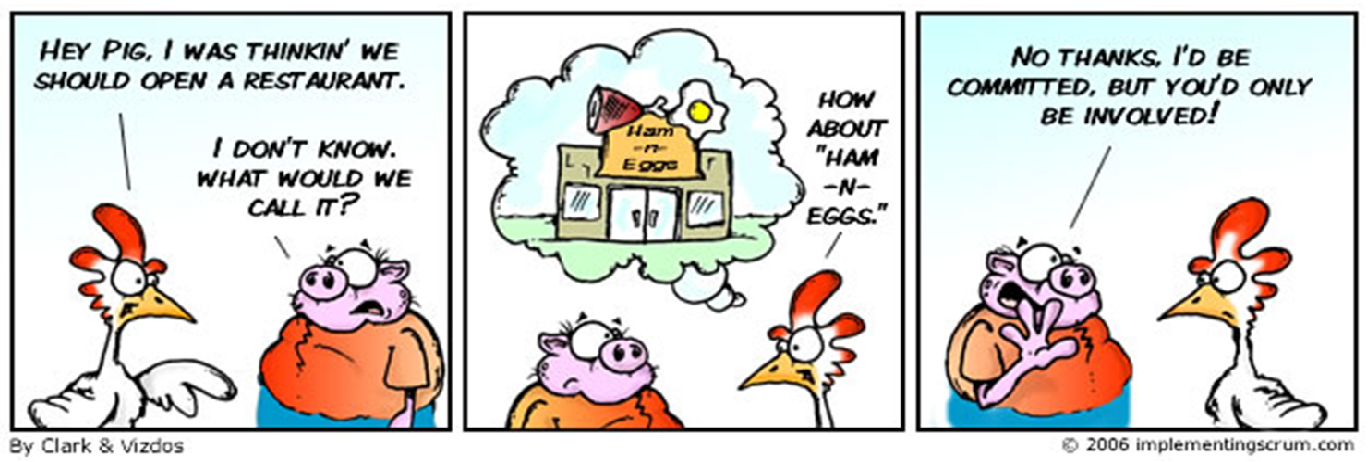
\includegraphics[width=1.20\textheight]{sc2.png}}
\end{frame}

\begin{frame} \frametitle{Роли в Scrum}
	\centerline{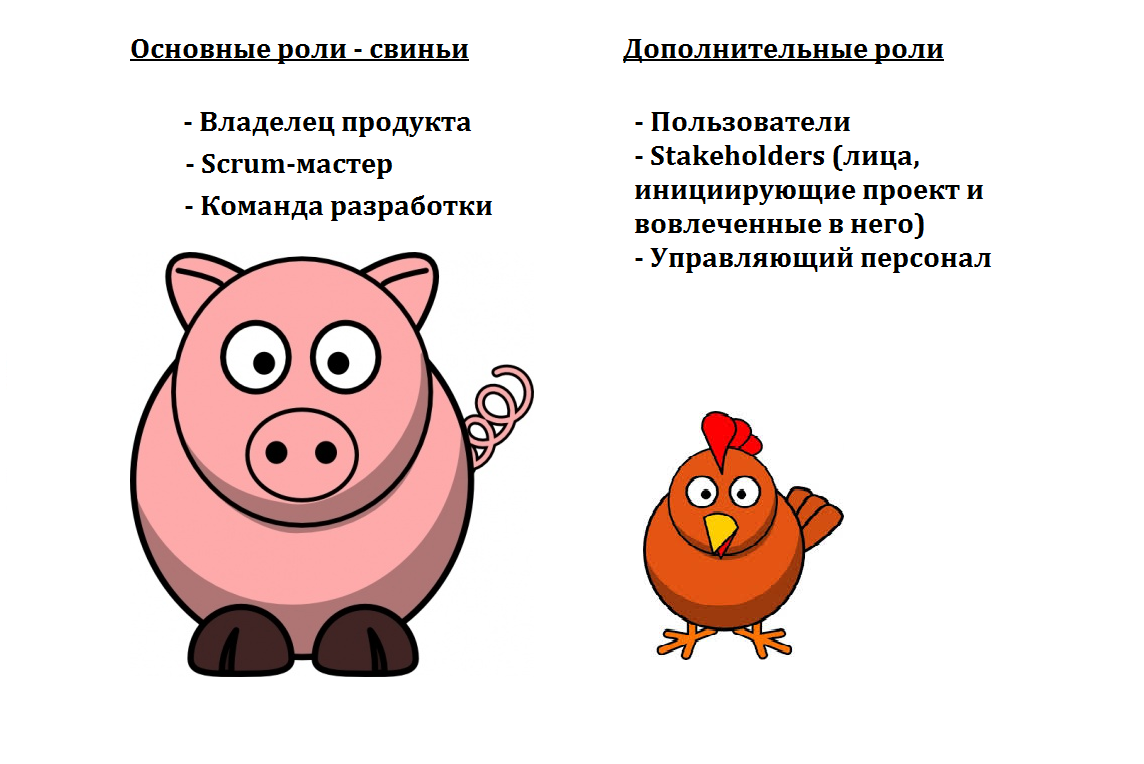
\includegraphics[width=1.50\textheight]{sc3.png}}
\end{frame}

\lecturenotes
По методике Scrum в производственном процессе есть определённые роли, разбитые на 2 группы \alert{«свиней»} и \alert{«кур»}. Эти названия были использованы из-за шутки.
Свинья идёт по дороге. Курица смотрит на неё и говорит: «А давай откроем ресторан!» Свинья смотрит на курицу и отвечает: «Хорошая идея, и как ты хочешь его назвать?» Курица думает и говорит: «Почему бы не назвать <<Яичница с беконом>>? <<Так не пойдёт>>, — отвечает свинья, — ведь тогда мне придётся полностью посвятить себя проекту, а ты будешь вовлечена только частично».

Свиньи создают продукт, тогда как куры заинтересованы, но не настолько — ведь им всё равно, будет ли проект удачным или нет, на них это мало отразится. Требования, пожелания, идеи и влияние кур принимаются во внимание, но им не разрешают непосредственно включаться в ход скрам-проекта~\cite[с.~54--56]{Рубин}.

Основные роли (Core roles) в методологии Scrum («Свиньи»):
\begin{itemize}
	\item \alert{Скрам-мастер} (Scrum Master) — проводит совещания (Scrum meetings) следит за соблюдением всех принципов скрама, разрешает противоречия и защищает команду от отвлекающих факторов. Данная роль не предполагает ничего иного, кроме корректного ведения скрам-процесса
	\item Руководитель проекта скорее относится к \alert{владельцу продукта} и не должен фигурировать в качестве скрам-мастера
  \item \alert{Владелец продукта (Product Owner)} — представляет интересы конечных пользователей и других заинтересованных в продукте сторон
  \item \alert{Команда Разработки (Development Team)} — кросс-функциональная команда разработчиков проекта, состоящая из специалистов разных профилей: тестировщиков, аналитиков, архитекторов, программистов и т.д. Размер команды в идеале составляет от 3 до 9 человек. Команда является единственным полностью вовлечённым участником разработки и отвечает за результат как единое целое. Никто, кроме команды, не может вмешиваться в процесс разработки на протяжении спринта
\end{itemize}
Дополнительные роли (Ancillary roles) в методологии скрам («Куры»):
\begin{itemize}
	\item Клиенты, продавцы (Stakeholders) — лица, которые инициируют проект и для кого проект будет приносить выгоду. Они вовлечены в Scrum только во время обзорного совещания по спринту (Sprint Review)
	\item Управляющие (Managers) — люди, которые управляют персоналом
	\item Эксперты-консультанты (Consulting Experts)~\cite{Scrum}
\end{itemize}

\subsection{Основные события Scrum}
\begin{frame} \frametitle {Основные события Scrum}
\begin {block} {Спринт}
\begin {itemize}
\itemСпринт служит \alert{ядром} Скрама. 

\item Это временной отрезок максимальной длительностью \alert{один месяц}, в течение которого команда создает функционирующий и  готовый к использованию и выпуску Инкремент продукта. 

\itemЖелательно сохранять \alert{неизменной} продолжительность Спринта на протяжении всего процесса разработки. 

\itemНовый Спринт начинается сразу после окончания предыдущего.
\end {itemize} 
\end {block}\end{frame}


\begin{frame} \frametitle{Scrum}
Cпринт - главная итерация Scrum.
\centerline{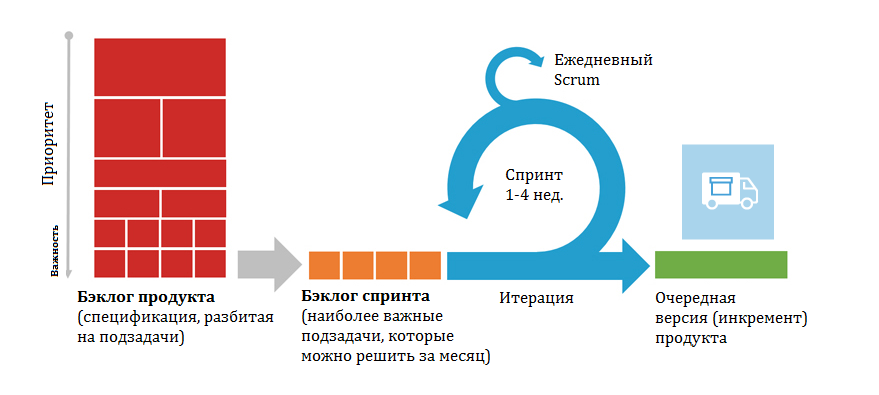
\includegraphics[height=0.6\textheight]{scrum.png}}
\end{frame} 


\begin{frame} \frametitle {Этапы спринта}
\leftline{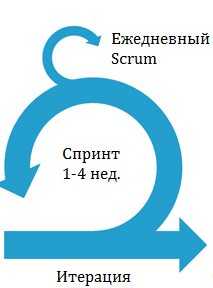
\includegraphics[height=0.6\textheight]{sprint.png}}
\begin{flushright}
\begin{itemize}
\item Планирование Спринта
\item Ежедневный Scrum
\item Разработка и Тестирования
\item Обзор Спринта
\item Ретроспектива Спринта. 
\end {itemize}
\end{flushright}
\end{frame}
\lecturenotes
\begin {block}
Спринт служит ядром Скрама. Это временной отрезок максимальной  длительностью один месяц, в течение которого      команда создает функционирующий и  готовый к использованию и выпуску Инкремент продукта. Желательно сохранять неизменной продолжительность Спринта на протяжении всего  процесса разработки. Новый Спринт начинается сразу после окончания предыдущего. Спринт состоит из Планирования Спринта, Ежедневного Скрама, разработки, Обзора Спринта и Ретроспективы Спринта~\cite{Scrum}. 
\end {block}


\begin{frame} \frametitle {Планирование спринта}
Происходит в начале новой итерации Спринта.
\begin{itemize}
\item Из бэклога проекта выбираются задачи, обязательства по выполнению которых за спринт принимает на себя команда
\item Определяются \alert{критерии готовности} продукта (важнейший артефакт Scrum)
\item На основе выбранных задач создается бэклог спринта. Каждая задача оценивается в идеальных человеко-часах
\item Решение задачи не должно занимать более 12 часов или одного дня. При необходимости задача разбивается на подзадачи
\item Обсуждается и определяется, каким образом будет реализован этот объём работ
\end{itemize}
\end{frame}

\begin{frame} \frametitle{Scrum}
Планирование нового спринта начинается с анализа бэклога продукта.
\centerline{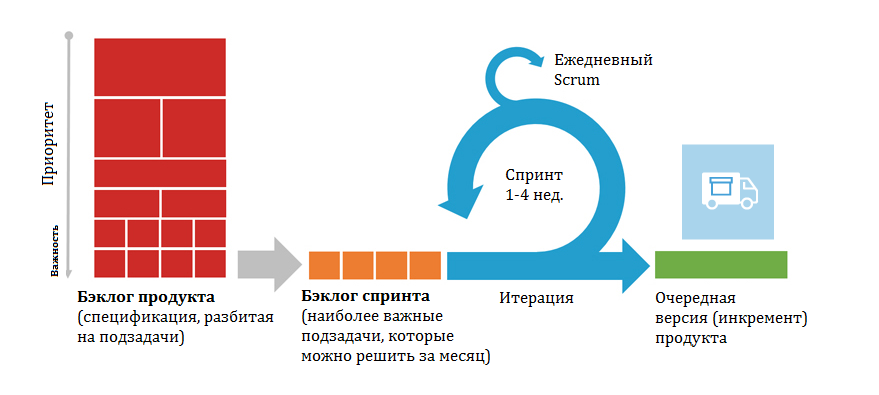
\includegraphics[height=0.6\textheight]{scrum.png}}
\end{frame} 

\begin{frame} \frametitle {Планирование спринта}

\begin{itemize}
\item Продолжительность совещания ограничена сверху 4---8 часами в зависимости от продолжительности итерации, опыта команды и т. п.
\item В 1 части совещания участвуют \alert {владелец проекта} и \alert{скрам команда}: они выбирают задачи из бэклога продукта;
\item В 2 части участвует \alert{только команда}: её участники обсуждают технические детали реализации, наполняют бэклог спринта.
\end {itemize}
\end{frame}

\lecturenotes
Планирование спринта (Sprint Planning Meeting) происходит в начале новой итерации Спринта.
\begin{itemize}
\item Из бэклога проекта выбираются задачи, обязательства по выполнению которых за спринт принимает на себя команда
\item На основе выбранных задач создается бэклог спринта. Каждая задача оценивается в идеальных человеко-часах
\item Решение задачи не должно занимать более 12 часов или одного дня. При необходимости задача разбивается на подзадачи
\item Обсуждается и определяется, каким образом будет реализован этот объём работ
\item Продолжительность совещания ограничена сверху 4—8 часами в зависимости от продолжительности итерации, опыта команды и т. п.
\item (первая часть совещания) Участвует \alert {владелец проекта} и \alert{скрам команда}: выбирают задачи из бэклога продукта
\item (вторая часть совещания) Участвует \alert{только команда}: обсуждают технические детали реализации, наполняют бэклог спринта~\cite{Scrum}
\end{itemize}



\begin{frame} \frametitle{Ежедневное совещание (ежедневный Scrum)}
Требования:
\begin{itemize}
\item Начинается точно вовремя;
\item Все могут наблюдать, но только «свиньи» говорят;
\item Длится не более 15 минут;
\item Проводится в одном и том же месте в течение спринта.
\end{itemize}
\end{frame}
\lecturenotes
\alert{Ежедневное совещание (ежедневный Scrum)}
\begin {block} {Требования}
\begin{itemize}
\item Начинается точно вовремя;
\item Все могут наблюдать, но только «свиньи» говорят;
\item Длится не более 15 минут;
\item Проводится в одном и том же месте в течение спринта.
\end{itemize}
\end {block}
\end{frame}

\begin{frame} \frametitle{Ежедневное совещание}
\begin {block} {В течение совещания каждый член команды отвечает на 3 вопроса:}
\begin{itemize}
\item Что я сделал с момента прошлой встречи для того, чтобы помочь команде разработки достигнуть цели спринта?
\item Что я сделаю сегодня для того, чтобы помочь команде разработки достичь цели спринта?
\item Вижу ли я препятствия для себя или команды разработки, которые могли бы затруднить достижение цели спринта? 
\end{itemize}
\end {block}
\end{frame}

\begin {block} {В течение ежедневного совещания каждый член команды отвечает на 3 вопроса:}
\begin{itemize}
\item Что я сделал с момента прошлой встречи для того, чтобы помочь Команде Разработки достигнуть Цели Спринта?
\item Что я сделаю сегодня для того, чтобы помочь Команде Разработки достичь Цели Спринта?
\item Вижу ли я препятствия для себя или Команды Разработки, которые могли бы затруднить достижение Цели Спринта? (Над решением этих проблем работает скрам мастер. Обычно это решение проходит за рамками ежедневного совещания и в составе лиц, непосредственно затронутых данным препятствием)

\lecturenotes
Ежедневное совещание (Daily Scrum meeting) должно отвечать следующим требованиям:
\begin{itemize}
\item начинается точно вовремя;
\item все могут наблюдать, но только «свиньи» говорят;
\item длится не более 15 минут;
\item проводится в одном и том же месте в течение спринта.
\end{itemize}
В течение совещания каждый член команды отвечает на 3 вопроса.
\begin{itemize}
\item Что я сделал с момента прошлой встречи для того, чтобы помочь Команде Разработки достигнуть Цели Спринта?
\item Что я сделаю сегодня для того, чтобы помочь Команде Разработки достичь Цели Спринта?
\item Вижу ли я препятствия для себя или Команды Разработки, которые могли бы затруднить достижение Цели Спринта? Над решением этих проблем работает скрам мастер. Обычно это решение проходит за рамками ежедневного совещания и в составе лиц, непосредственно затронутых данным препятствием~\cite{Scrum}
\end{itemize}
\end {block}


\begin{frame} \frametitle{Scrum}
Ежедневный Scrum есть повторение спринта в масштабе суток.
\centerline{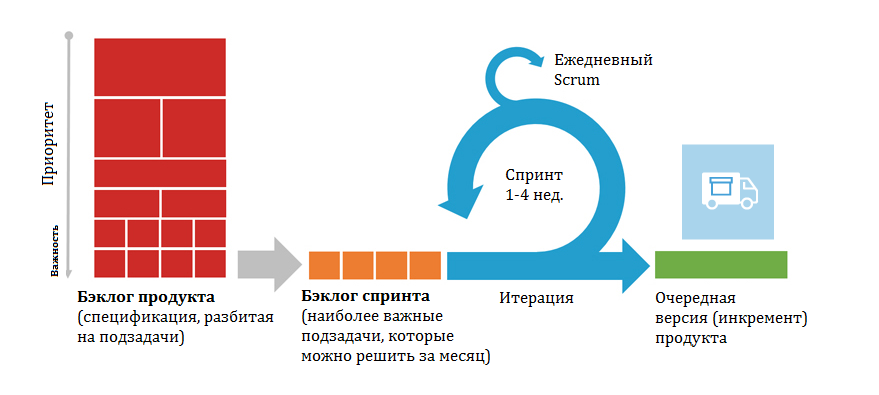
\includegraphics[height=0.6\textheight]{scrum.png}}
\end{frame} 

\begin{frame} \frametitle{Скрам над скрамом}
Проводится после ежедневного скрам-совещания и позволяет скрам-командам обсуждать пересечения в общих областях и взаимной интеграции. Рассматриваются такие вопросы как:
\begin {block}{}
\begin{itemize}
\item Что каждая команда сделала с момента предыдущего ежедневного совещания?
\item Что каждая команда сделает к следующему ежедневному совещанию?
\item Есть ли проблемы, мешающие или замедляющие работу каждой команды?
\item Нужно ли другой команде сделать что-то из задач вашей команды?
\end{itemize}
\end {block}
\end{frame}

\lecturenotes
\alert{Скрам над скрамом} проводится после ежедневного скрам-совещания. 
Позволяет нескольким скрам-командам обсуждать работу, фокусируясь на общих областях и взаимной интеграции. Повестка та же, что и на ежедневном скрам-совещании плюс следующие вопросы:
\begin {block}{}
\begin{itemize}
\item Что каждая команда сделала с момента предыдущего ежедневного совещания?
\item Что каждая команда сделает к следующему ежедневному совещанию?
\item Есть ли проблемы, мешающие или замедляющие работу каждой команды?
\item Нужно ли другой команде сделать что-то из задач вашей команды~\cite{Scrum}?
\end{itemize}
\end {block}
\end{frame}

\begin{frame} \frametitle{Обзор итогов спринта}
Проводится в конце спринта:
\begin{itemize}
\item Команда демонстрирует прирост функциональности продукта всем заинтересованным лицам (очередой \alert{инкремент})
\item Привлекается максимальное количество зрителей
\item Все члены команды участвуют в демонстрации (один человек на демонстрацию или каждый показывает, что сделал за спринт)
\item Нельзя демонстрировать незавершенную функциональность
\item Ограничена четырьмя часами
\end{itemize}
\end{frame}
\lecturenotes
Обзор итогов спринта (Sprint review meeting)
\begin {block}
Проводится в конце спринта. По своей сути данный этап является рефлексией всего спринта.\end {block}
\begin{itemize}
\item Команда демонстрирует прирост функциональности продукта всем заинтересованным лицам
\item Привлекается максимальное количество зрителей
\item Все члены команды участвуют в демонстрации (один человек на демонстрацию или каждый показывает, что сделал за спринт)
\item Нельзя демонстрировать незавершенную функциональность.
\item Ограничена четырьмя часами в зависимости от продолжительности итерации и прироста функциональности продукта~\cite{Scrum}
\end{itemize}


\begin{frame} \frametitle{Ретроспективное совещание}
Проходит после обзора \alert{итогов спринта}, но уже с акцентом на будущие задачи. Члены команды высказывают своё мнение о прошедшем спринте и отвечают на два основных вопроса:
\begin{block}{}
\begin{itemize}
\item Что было сделано хорошо в прошедшем спринте?
\item Что надо улучшить в следующем?
\end{itemize}
\end{block}
\end{frame}


\begin{frame} \frametitle{Ретроспективное совещание}
Команда выполняет \alert{улучшение процесса разработки}(решает вопросы и фиксирует удачные решения) путём
\begin{itemize}
\item демонстрации своих результатов 
\item нельзя демонстрировать \alert{незавершенную функциональность}
\end{itemize}
Совещание ограничено \alert{четырьмя часами} в зависимости от продолжительности итерации и прироста функциональности продукта.
\end{frame}

\lecturenotes
Ретроспективное совещание (Retrospective meeting) также проводится в конце спринта, но уже с акцентом на будущие задачи. Члены команды высказывают своё мнение о прошедшем спринте и отвечают на два основных вопроса:
\begin{itemize}
\item Что было сделано хорошо в прошедшем спринте?
\item Что надо улучшить в следующем?
\item Все члены команды участвуют в демонстрации (один человек на демонстрацию или каждый показывает, что сделал за спринт).
\item Нельзя демонстрировать незавершенную функциональность.
\item Ограничена четырьмя часами в зависимости от продолжительности итерации и прироста функциональности продукта.
\end{itemize}
Таким образом, команда выполняют улучшение процесса разработки (решает вопросы и фиксирует удачные решения). Данный этап ограничен одним-тремя часами~\cite{Scrum}.


\subsection{Артефакты Скрама}

\begin{frame} \frametitle{Agile}
Артефакты (бэклог продукта, спринта и инкремент) в Scrum
\centerline{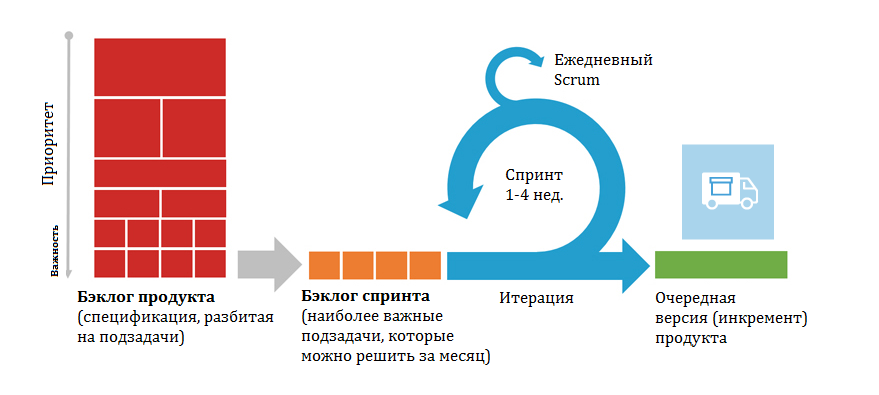
\includegraphics[height=0.6\textheight]{scrum.png}}
\end{frame}

\begin{frame} \frametitle{{Артефакты Скрама}}
\begin {block} {Функции артефактов} 
\begin{itemize}
\item Отражая работу или ценность, артефакты Скрама также обеспечивают \alert{прозрачность} и
создают новые возможности для \alert{инспекции} и \alert{адаптации}. 
\item Артефакты Скрама призваны
обеспечить максимальную прозрачность ключевой информации, чтобы все участники
процесса обладали ее одинаковым пониманием.
\end{itemize}
\end{block} 
\end {frame} 

\lecturenotes
Отражая работу или ценность, артефакты Скрама также обеспечивают прозрачность и
создают новые возможности для инспекции и адаптации. Артефакты Скрама призваны
обеспечить максимальную прозрачность ключевой информации, чтобы все участники
процесса обладали ее одинаковым пониманием~\cite{Scrum}.

\begin{frame} \frametitle {Бэклог продукта} 
\begin {block} {Определение}
\alert{Бэклог продукта} – это упорядоченный список всего, что может понадобиться в продукте.
Это единственный источник требовании для любого вида изменений, которые могут быть
внесены в продукт. 
\end{block} 
Ответственность за бэклог продукта, включая его содержание,
доступность и упорядочивание элементов, несет \alert{владелец продукта}.
\end {frame}
 


\begin{frame} \frametitle {Свойства Бэклога продукта} 
\begin{itemize}
\item Никогда не бывает \alert{полным}. Его начальный вариант содержит только
изначально известные и наиболее понятные требования

\item Изменяется по мере обновления продукта и
изменений внешних факторов 

\item Поэтому продукт остается \alert{актуальным,
конкурентоспособным и приносящим пользу}
\end{itemize}
\begin{block}{Следствие} Бэклог существует до тех пор, пока существует продукт.
\end{block} 
\end {frame} 

\lecturenotes
Бэклог Продукта содержит данные, определяющие необходимость изменений в
последующих выпусках продукта. К числу таких данных могут относиться новые
характеристики или новые функции продукта, требования, информация о путях
усовершенствования продукта и устранения дефектов. Каждый элемент Бэклога Продукта
должен содержать описание, номер позиции в Бэклоге, оценку объема работы и ценность.
По мере получения обратной связи от рынка – когда продуктом начинают пользоваться и
он приносит прибыль – Бэклог Продукта становится все более объемным и
исчерпывающим. К его изменениям также могут привести перемены в мире бизнес‐
требований, технологий, условий рынка. Поскольку требования постоянно меняются,
Бэклог Продукта остается живым артефактом.

Когда над одним продуктом работают несколько Скрам‐команд, для описания всех
предстоящих работ используется только один Бэклог Продукта. При этом его элементы
могут быть сгруппированы по атрибутам.

Уточнение Бэклога Продукта – это деятельность, направленная на уточнение,
оценку и упорядочивание элементов в Бэклоге Продукта. Речь идет о непрерывном
процессе, в рамках которого Владелец Продукта и Команда Разработки обсуждают детали элементов Бэклога Продукта, тем самым проверяя и пересматривая эти элементы. Скрам‐команда решает, как и когда должно производиться Уточнение Бэклога Продукта. Этот
процесс обычно занимает не более одной десятой от доступного времени Скрам‐команды. При этом
элементы Бэклога Продукта в любой момент времени могут быть изменены как самим
Владельцем Продукта, так и по его указанию.

Желательно, чтобы элементы Бэклога Продукта, расположенные сверху, были более
детализированными и понятными по сравнению с расположенными ниже элементами.
Чем детальнее описание элементов Бэклога Продукта, тем точнее может быть их оценка. В
свою очередь, чем ниже находятся элементы в Бэклоге Продукта, тем меньше они
детализированы.

Детализация же элементов Бэклога Продукта, над которыми Команда Разработки будет
работать во время следующего Спринта, предполагает, что каждый из элементов может
быть потенциального готов в течение Спринта так, что не остается никакой другой работы,
чтобы подготовить продукт к выпуску.

Элементы Бэклога Продукта, которые могут быть доведены Командой Разработки до
состояния готовности в течение Спринта считаются Подготовленными для следующего
Планирования Спринта. Данная степень прозрачности может быть достигнута посредством
уточнения элементов Бэклога Продукта---с помощью описанных выше активностеи.
Команда Разработки отвечает за окончательные оценки задач. При этом Владелец
Продукта может помочь Команде Разработки лучше понять суть работы~\cite{Scrum}.



\begin{frame} \frametitle {Бэклог cпринта}
\begin {block}{Бэклог спринта }
это набор элементов бэклога продукта, выбранный для исполнения в текущем спринте. Он включает в себя 
\begin{itemize}
	\item план разработки инкремента продукта
	\item план достижения цели спринта
\end{itemize}
\end{block} 
Бэклог Спринта является \alert{прогнозом} команды разработки касающегося
функциональности, которая станет следующим инкрементом, и работы, которую
надо выполнить для соответствия критериям готовности.
\end {frame} 

\begin{frame} \frametitle{Бэклог спринта}

 \alert{Бэклог Спринта} отображает весь объем работ, который команда разработки считает
необходимым для достижения цели спринта.
\centerline{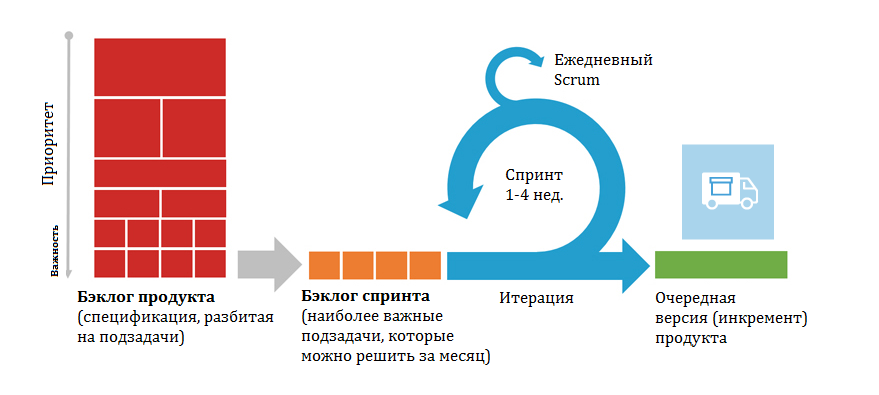
\includegraphics[height=0.6\textheight]{scrum.png}}
\end{frame}

\lecturenotes
Бэклог спринта – это набор элементов бэклога продукта, выбранный для исполнения в
текущем спринте. Он включает в себя как план разработки инкремента продукта, так и
план достижения цели спринта.
Бэклог спринта является прогнозом команды разработки. Данный прогноз касается
функциональности, которая станет следующим инкрементом, и работы, которую
необходимо выполнить для соответствия критериям готовности.
бэклог спринта отображает весь объем работ, который команда разработки считает
необходимым для достижения цели спринта.
Поскольку Бэклог спринта представляет достаточно детальный план, прогресс может
быть определен в рамках ежедневного скрама. Работая над выполнением плана, команда
Разработки узнает больше о необходимых шагах для достижения цели спринта.
Следовательно, бэклог спринта претерпевает изменения, а в ходе выполнения плана
появляется новый спектр работ.
Команда разработки добавляет появившиеся задачи в бэклог спринта. По мере
выполнения и завершения работ обновляется оценка оставшейся работы. Элементы плана
могут быть удалены, если команда считает, что они потеряли актуальность. Однако во
время спринта изменять бэклог спринта может только команда разработки.
Бэклог спринта принадлежит исключительно команде разработки и служит наглядным
представлением реального объема работ, который планирует выполнить команда
разработки в течение спринта~\cite{Scrum}.

\begin{frame} \frametitle {Отслеживание прогресса cпринта}

\begin{itemize}
\item В Scrum в любой момент времени \alert{может быть подсчитан} 
объем работ, оставшийся в бэклоге  спринта. Отслеживание оставшегося объема задач необходимо команде разработки, чтобы \alert{правильно оценить} вероятность достижения цели спринта и управлять ходом исполнения работ. 

\item Более подробно об отслеживании прогресса можно судить по \alert{критериям готовности}, также являющимися одним из артефактов Scrum.
\end{itemize} 
\end{frame} 
\lecturenotes
В Scrum в любой момент времени может быть подсчитан 
объем работ, оставшийся в Бэклоге Спринта. Отслеживание оставшегося объема задач необходимо Команде Разработки, чтобы
правильно оценить вероятность достижения Цели Спринта и управлять ходом исполнения работ. Более подробно об отслеживании прогресса можно судить по Критериям Готовности, также являющимися одним из артефактов Scrum~\cite{Scrum}.

\begin{frame} \frametitle {Инкремент}
\begin {block}{Инкремент}
это сумма, как всех элементов Бэклога Продукта, завершенных во время
Спринта, так и всех инкрементов предыдущих Спринтов.
\end{block} 
К концу спринта инкремент должен быть готов, что подразумевает его соответствие
критериям готовности скрам‐команды и готовность к использованию.
\end {frame}

\begin{frame} \frametitle{Инкремент}
Инкремент должен быть готовым к использованию вне зависимости от решения владельца продукта его выпускать или повременить.
\centerline{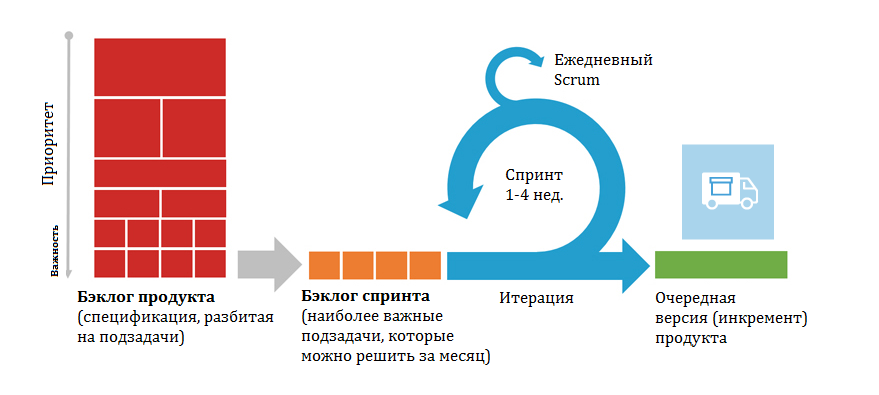
\includegraphics[height=0.6\textheight]{scrum.png}}
\end{frame} 
\lecturenotes
Инкремент – это сумма, как всех элементов Бэклога Продукта, завершенных во время
Спринта, так и всех инкрементов предыдущих Спринтов.
К концу Спринта Инкремент должен быть Готов, что подразумевает его соответствие
критериям Готовности Скрам‐команды и готовность к использованию. Он должен быть готовым к использованию вне зависимости от решения Владельца Продукта его выпускать или повременить~\cite{Scrum}.


\subsection{Критерии Готовности}

\begin{frame} \frametitle {Критерии Готовности}

\begin{itemize}
	\item Понимание состояния готовности элементов Бэклога или Инкремента является
обязательным для членов команды. 
  \item Различные Скрам‐команды могут отличаться определением состояния готовности
 \item Участники каждой команды должны понимать общее значение выполненной работы
\begin{block}{}
Последнее условие служит одним из условий обеспечения \alert{прозрачности}(понятности и однозначности для всех участников проекта) и используется для принятия готовой работы над \alert{Инкрементом продукта}.
\end{block}
\end{itemize}
\end {frame}


\begin{frame} \frametitle {Критерии Готовности}
\begin{itemize}
	\item Помогают команде разработки понять, \alert{сколько элементов бэклога продукта следует взять в Спринт} во время планирования.
 \item Назначение каждого Спринта---обеспечить Инкремент потенциально готовой к выпуску функциональности. При этом
данная функциональность должна соответствовать критериям готовности скрам‐команды в текущий момент.
 \item Команда Разработки предоставляет Инкремент функциональности продукта каждый Спринт. Поскольку этот Инкремент готов к использованию, Владелец Продукта может \alert{принять решение о его немедленном выпуске}.
\end{itemize}
\end {frame}
\lecturenotes
Понимание состояния готовности элементов бэклога или инкремента является
обязательным для членов команды. различные скрам‐команды могут отличаться
определением состояния готовности.
Однако участники каждой команды должны понимать общее значение выполненной
работы. Данное понимание служит одним из условий обеспечения прозрачности и
используется для принятия готовой работы над инкрементом продукта.
Эти же критерии помогают команде разработки узнать, сколько элементов Бэклога
Продукта следует взять в спринт во время планирования. Назначение каждого спринта –
обеспечить инкремент потенциально готовой к выпуску функциональности. При этом
данная функциональность соответствует критериям готовности скрам‐команды в текущий
момент.
Команда разработки предоставляет инкремент функциональности продукта каждый
Спринт. Поскольку этот инкремент готов к использованию, владелец продукта может
принять решение о его немедленном выпуске~\cite{Scrum}.

\subsection{Прозрачность Артефактов}
\begin{frame}\frametitle {Прозрачность Артефактов}

\begin{itemize}
\item Scrum опирается на прозрачность. Это одно из самых важных свойств методологии. Оно определяется \alert{общими для всех} стандартами. 
\item Решения о получении оптимальной ценности и управлении рисками основываются на состоянии артефактов (бэклоги проекта, спринта, ежедневного спринта, критерии готовности)
\end{itemize}
\end {frame}

\begin{frame}\frametitle {Прозрачность Артефактов}

\begin{itemize}
\item Под состоянием артефактов подразумевают степень их прозрачности (понимания их всеми участниками проекта)
\item При неполной прозрачности решения могут быть ошибочными, ценность снижена, а риски увеличены. Поэтому Скрам‐мастер должен сотрудничать со всеми вовлеченными сторонами – Владельцем Продукта, Командой Разработки и другими – чтобы понимать степень прозрачности артефактов.
\item Прозрачность появляется не сразу, но это \alert{конечная цель}
\end{itemize}
\end {frame}
\lecturenotes
Скрам опирается на прозрачность. Это одно из самых важных свойств методологии. Решения о получении оптимальной ценности и управлении рисками основываются на состоянии артефактов. Под состоянием артефактов подразумевают степень их
прозрачности – ключевой фактор прочности этих решений. При неполной прозрачности решения могут быть ошибочными, ценность снижена, а риски увеличены. Поэтому Скрам‐мастер должен сотрудничать со всеми вовлеченными
сторонами – Владельцем Продукта, Командой Разработки и другими – чтобы понимать
степень прозрачности артефактов. В условиях неполной прозрачности, Скрам‐мастер должен помочь внедрению практик,
которые наиболее эффективно эти условия устранят. Скрам‐мастер может определить неполную прозрачность путем инспекции артефактов, обнаружения повторяющихся шаблонов, определения разницы между ожидаемым и полученным результатом, а также – путем анализа. Анализу подлежит объем ранее озвученной информации, исходящей от вовлеченных в процесс сторон.
Задача Скрам‐мастера – увеличить прозрачность артефактов, работая со Скрам‐командой организацией. Данная работа обычно включает обучение, убеждение и организационные изменения. Прозрачность – это путь, предполагающий постепенное
становление, и этот путь необходимо пройти~\cite{Scrum}.



\begin{thebibliography}{99}
\bibitem{Рубин} Рубин К. Основы Scrum: Практическое руководство по гибкой разработке ПО. М.: Вильямс,  2016 . — 544 с. 
Кеннет Рубин. 
\bibitem{Winston} \href{http://www.cs.umd.edu/class/spring2003/cmsc838p/Process/waterfall.pdf}{Dr. Winston W. Roуce. MANAGING THE DEVELOPMENT OF LARGE SOFTWARE SYSTEMS}
\bibitem{MethodolyComparison} \href{https://www.cms.gov/Research-Statistics-Data-and-Systems/CMS-Information-Technology/XLC/Downloads/SelectingDevelopmentApproach.pdf}
\bibitem{Boehm} \href{http://csse.usc.edu/TECHRPTS/1988/usccse88-500/usccse88-500.pdf}
\end{thebibliography}
\bibitem{Scrum} \href{http://www.scrumguides.org/scrum-guide.html}
\bibitem{Agile} \href{http://agilemanifesto.org/}
\end{thebibliography}


\end{document}

%%% Local Variables: 
%%% mode: TeX-pdf
%%% TeX-master: t
%%% End: 
